\section{Durchführung}
\label{sec:Durchführung}

% Was wurde gemessen bzw. welche Größen wurden variiert?

\begin{figure}
    \centering
    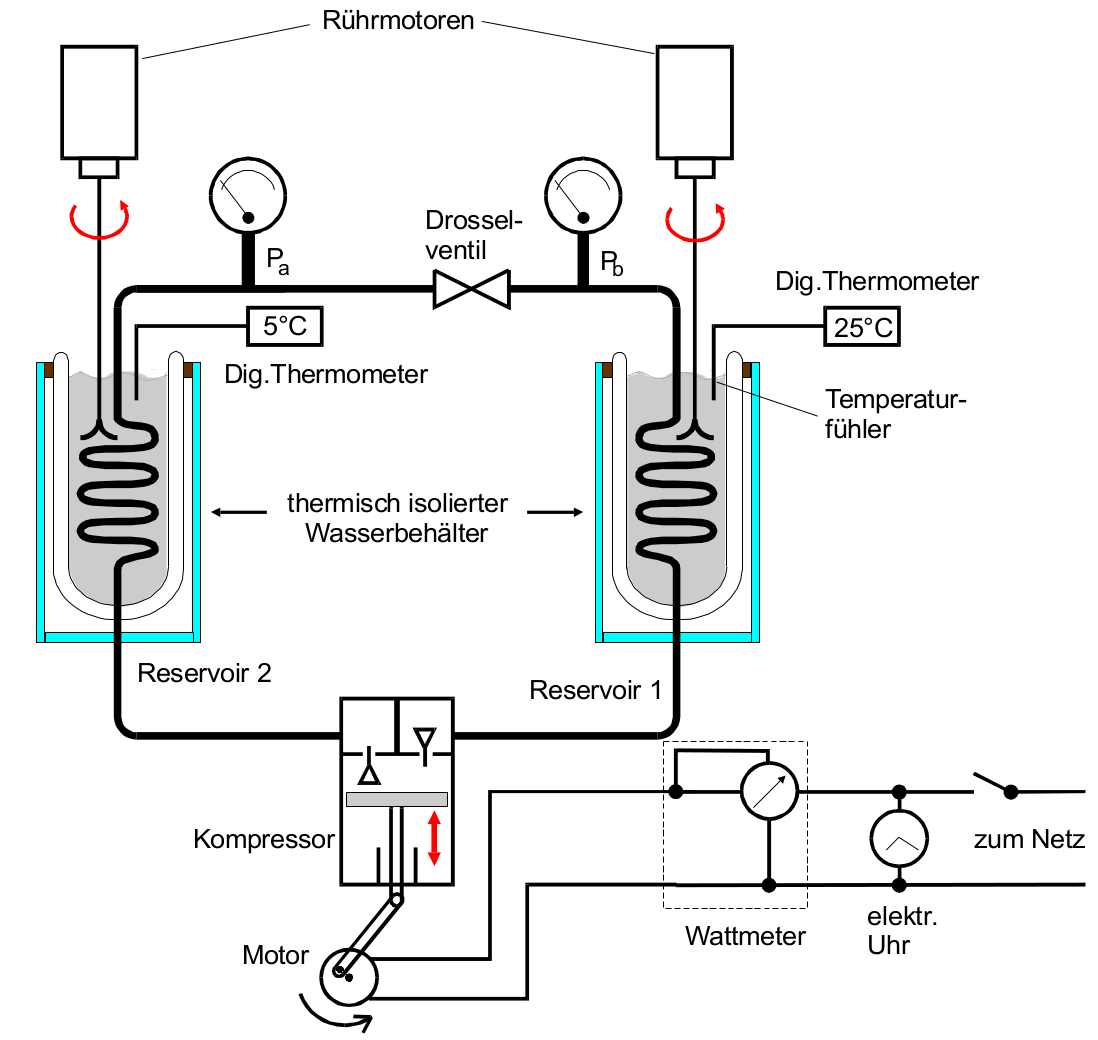
\includegraphics[width=\textwidth/2]{images/skizze_2.png}
    \caption{Aufbau der Wärmepumpe\cite{V206}}
    \label{fig:skizze_2}
\end{figure}

Zunächst wird eine Wärmepumpe wie in \autoref{fig:skizze_2} aufgebaut.
Die Reservoirs werden mit je 3 Litern Wasser gefüllt, wobei beide Reservoire ungefähr die gleiche Temperatur aufweisen sollten.
Dann werden die Rührstäbe angeschaltet, damit sich die Wärme gleichmäßig verteilt.
Sobald der Kompressor angeschaltet wird, fängt die Wärmepumpe an zu arbeiten.
Nun werden im Minutentakt folgende Größen abgelesen und notiert:
\begin{itemize}
    \item verstrichene Zeit $t$ seit dem Anschalten des Kompressors
    \item Temperatur $T_1$ im Reservoir 1
    \item Temperatur $T_2$ im Reservoir 2
    \item Druck $p_a$ im Reservoir 1
    \item Druck $p_b$ im Reservoir 2
    \item elektrische Leistung $N_\text{el}$ des Kompressors
\end{itemize}

Sobald in Reservoir 1 eine Temperatur von $\SI{50}{\degree\celsius}$ erreicht ist, wird der Kompressor abgeschaltet und die Messung ist abgeschlossen.